\documentclass[a4paper,12pt]{amsart}

\usepackage[
  margin=30mm,
  marginparwidth=25mm,     % + <- Width of your marginpar
  marginparsep=2mm,       % + <- Gap between text block and marginpar
%  paperwidth=107.95mm,
%  paperheight=174.63mm,
  bottom=25mm,
  ]{geometry}


\usepackage{graphicx} % Required for inserting images
\usepackage{amsmath} % For mathematical equations
\usepackage{amssymb} % For mathematical symbols
\usepackage{braket} % For Dirac notation
\usepackage{tikz} % For drawing circuits
\usepackage{circuitikz} % For classical circuit diagrams
\usetikzlibrary{quantikz} % For quantum circuit diagrams
\usetikzlibrary{angles, quotes}
\usepackage{hyperref} % For clickable links and references


\title{Capstone: Spectral Methods for Variational Quantum Linear Solvers}
\author{Adilet Akimshe}
\date{January 2026}

\begin{document}

\begin{abstract}
We investigate how the choice of polynomial basis in spectral collocation methods affects the Pauli term count of the resulting system matrix in Variational Quantum Linear Solvers (VQLS). Solving linear systems is fundamental to scientific computing, and VQLS offers a promising near-term quantum approach compatible with Noisy Intermediate-Scale Quantum (NISQ) devices. A key bottleneck in VQLS efficiency is the Pauli term count in the decomposition of the system matrix, which directly determines measurement overhead and circuit complexity. Through a sequence of four numerical experiments on second-order ordinary differential equations, we show that the standard monomial (Case~A) basis saturates all $4^n$ available Pauli strings for an $n$-qubit system, while a basis-change identity reduces this problem to a linear program (LP) over the collocation matrix. The global LP always recovers the identity matrix $M^* = I_N$ as the unique optimum---a single Pauli string regardless of the differential operator, domain, or boundary conditions---but this collapses the quantum problem into a classically trivial state-preparation task. A \emph{monic LP} variant, restricting the basis to lower-triangular coefficient matrices with unit diagonal, provides a principled middle ground: it reduces Hadamard-test overhead by factors of $3$--$7\times$ while preserving a non-trivial quantum system. These results sharply characterize the trade-off between Pauli efficiency and quantum non-triviality in collocation-based quantum linear solvers.
\end{abstract}

\maketitle

\tableofcontents

\section{Introduction}
Quantum computers represent a paradigm shift in computational technology, leveraging the principles of quantum mechanics to process information in fundamentally different ways than classical computers. Unlike classical bits that exist in definite states of 0 or 1, quantum bits (qubits) can exist in superpositions of states, enabling quantum algorithms to explore multiple solution paths simultaneously. This property, combined with quantum entanglement and interference, allows quantum computers to potentially solve certain problems exponentially faster than their classical counterparts \cite{nielsen2011quantum, hidary2021quantum}.

The development of quantum algorithms for solving linear systems of equations has garnered significant attention, as linear algebra problems form the backbone of scientific computing, machine learning, and optimization. In particular, quantum spectral methods have emerged as a powerful approach for solving differential equations with complexity that scales only poly-logarithmically in the system dimension \cite{childs2020spectral}. Variational Quantum Linear Solvers (VQLS) represent a promising near-term approach that is compatible with current Noisy Intermediate-Scale Quantum (NISQ) devices.

\subsection{History}
%add famous papers that I did not cite
The concept of quantum computing was first proposed by Richard Feynman in 1982, who suggested that quantum systems could be simulated more efficiently using quantum computers rather than classical ones \cite{nielsen2011quantum}. David Deutsch formalized this idea in 1985 by describing a universal quantum computer. The field gained significant momentum in 1994 when Peter Shor developed his famous algorithm for integer factorization, demonstrating that quantum computers could solve certain problems exponentially faster than classical computers \cite{nielsen2011quantum, yanofsky2008quantum}.

The late 1990s and early 2000s saw the development of quantum error correction codes and the first experimental implementations of small quantum systems. Grover's search algorithm (1996) and the development of quantum simulation techniques further established the theoretical foundation of quantum computing \cite{nielsen2011quantum}.

In recent years, the focus has shifted toward NISQ devices and variational quantum algorithms. These algorithms, including the Variational Quantum Eigensolver (VQE) and VQLS, are designed to work within the constraints of current quantum hardware, which is limited by decoherence and gate errors \cite{hidary2021quantum, schuld2018supervised}. A comprehensive historical overview of quantum computing can be found in Chapter~1 of Nielsen and Chuang~\cite{nielsen2011quantum} and the introductory chapter of Hidary~\cite{hidary2021quantum}.

\section{Preliminaries}
%add that the content is taken from the textbook
%reference a few more textbooks
%you can add youtube videos in the appendix or supplementary
%reference specific pages in the textbooks for the interested readers
This section provides the foundational concepts necessary to understand the application of spectral methods to variational quantum linear solvers.

\subsection{Classical bits}
A classical bit is the fundamental unit of information in classical computing. It can exist in one of two discrete states: 0 or 1. These states typically correspond to physical quantities such as voltage levels in electronic circuits (e.g., low voltage = 0, high voltage = 1) or magnetic orientations in storage media.

Mathematically, we can represent a classical bit as an element of the set $\{0, 1\}$. Multiple bits can be combined to represent larger numbers or more complex information. For example, $n$ classical bits can represent $2^n$ different states, but can only be in one specific state at any given time.

The deterministic nature of classical bits means that reading or measuring a bit does not change its state—a 0 remains 0 and a 1 remains 1 after measurement. This property is fundamentally different from quantum bits, as we will see later. In essence, a classical bit is like a coin: either heads or tails up. A rigorous treatment of classical information and computation is given in Chapter~1 of~\cite{nielsen2011quantum}.

\subsection{Classical logical gates}
Classical logical gates are the building blocks of classical circuits. They perform Boolean operations on one or more input bits to produce output bits. The most common gates include:

\textbf{NOT gate:} Inverts the input bit. If input is 0, output is 1, and vice versa. This is the only non-trivial single-bit gate.

\textbf{AND gate:} Takes two inputs and outputs 1 only if both inputs are 1.

\textbf{OR gate:} Takes two inputs and outputs 1 if at least one input is 1.

\textbf{XOR gate (Exclusive-OR):} Takes two inputs and outputs 1 if the inputs are different.

\textbf{NAND gate:} The negation of AND; outputs 0 only if both inputs are 1.

These gates can be combined to create more complex operations. Importantly, NAND gates (and similarly NOR gates) are \textbf{universal}: any Boolean function can be implemented using only NAND gates. This property is crucial for building general-purpose computers \cite{nielsen2011quantum, yanofsky2008quantum}.

Classical gates are typically \textbf{irreversible}: given only the output, you cannot always determine the input (e.g., AND gate output of 0 could come from inputs 00, 01, or 10). This irreversibility results in an irretrievable loss of information \cite{nielsen2011quantum}.

Quantum gates, in contrast, are unitary (explained why below) and thus reversible. For a complete treatment of Boolean logic, classical gates, and their computational universality, see ~\cite[Chapter~1]{nielsen2011quantum}.

\subsection{Classical circuits}
Classical circuits are composed of logical gates connected in specific configurations to perform computational tasks. Information flows through the circuit from input registers, through various gate operations, to output registers. Classical circuits consist of wires (to carry information) and logic gates (to manipulate the information).

A classical circuit can be represented as a directed acyclic graph (DAG), where nodes represent gates and edges represent wires carrying bit values. The depth of a circuit is the length of the longest path from input to output, which relates to the time complexity of the computation.

Classical circuits allow for operations like FANIN (joining wires together via OR operation) and FANOUT (creating multiple copies of a bit). These operations are fundamental to classical computing but, as we will see, have no direct quantum analogs.

Classical circuits are the foundation of all modern digital electronics, from simple calculators to complex processors. They implement algorithms through sequences of logical operations, with the state of the system at each step being completely determined by the previous state and the gate operations \cite{nielsen2011quantum, yanofsky2008quantum}.

\textbf{Example: Half adder}
A canonical example of a classical circuit is the \textbf{half adder}, which adds two single-bit inputs $A$ and $B$ and produces a 2-bit result: a sum bit and a carry bit.

\begin{figure}[h]
\centering
\begin{circuitikz}
    \node[and port] at (4, 0.75) (AND) {};
    \node[xor port] at (4,-0.75) (XOR) {};
    % Input A: main wire, with branch down to XOR top input
    \draw (AND.in 1) -- ++(-3, 0) node[left] {$A$};
    \draw (AND.in 1) ++(-1.5, 0) node[circ]{} |- (XOR.in 1);
    % Input B: main wire, with branch up to AND bottom input
    \draw (XOR.in 2) -- ++(-3, 0) node[left] {$B$};
    \draw (XOR.in 2) ++(-2.5, 0) node[circ]{} |- (AND.in 2);
    % Output wires
    \draw (AND.out) -- ++(1.5, 0) node[right] {Carry $= A \wedge B$};
    \draw (XOR.out) -- ++(1.5, 0) node[right] {Sum $= A \oplus B$};
\end{circuitikz}
\caption{Half adder: a classical circuit computing the 2-bit sum of inputs $A$ and $B$. The AND gate produces the carry bit and the XOR gate produces the sum bit. Filled dots denote wire junctions; wire crossings without a dot are not connected.}
\label{fig:half_adder}
\end{figure}

\subsection{Qubits}
A qubit (quantum bit) is the fundamental unit of quantum information. Unlike classical bits, qubits can exist in superposition states—simultaneously being in both 0 and 1 states with certain probability amplitudes.

Mathematically, a qubit state is represented as a vector in a two-dimensional complex Hilbert space:
\begin{equation}
|\psi\rangle = \alpha|0\rangle + \beta|1\rangle
\end{equation}
where $\alpha$ and $\beta$ are complex amplitudes satisfying the normalization condition $|\alpha|^2 + |\beta|^2 = 1$ \cite{nielsen2011quantum, scherer2019mathematics}. The states $|0\rangle$ and $|1\rangle$ form an orthonormal basis (also called the computational basis), corresponding to the classical bit values.

When measured in the computational basis, the qubit collapses to either $|0\rangle$ with probability $|\alpha|^2$ or $|1\rangle$ with probability $|\beta|^2$. This measurement is probabilistic and irreversible—after measurement, the superposition is destroyed. For instance, a qubit in the state
\begin{equation}
|+\rangle = \frac{1}{\sqrt{2}}|0\rangle + \frac{1}{\sqrt{2}}|1\rangle
\end{equation}
yields 0 or 1 with equal probability (50\% each) when measured.

\textbf{Physical realizations:} Qubits can be realized in various physical systems:
\begin{itemize}
    \item Polarization states of photons
    \item Nuclear spin alignment in magnetic fields
    \item Electronic states of atoms (ground state $|0\rangle$ and excited state $|1\rangle$)
    \item Superconducting circuits
\end{itemize}

\textbf{The Bloch Sphere:} Any qubit state can be parameterized as:
\begin{equation}
|\psi\rangle = \cos\frac{\theta}{2}|0\rangle + e^{i\phi}\sin\frac{\theta}{2}|1\rangle
\end{equation}
where $\theta$ and $\phi$ are real numbers defining a point on the unit three-dimensional sphere (see Figure \ref{fig:bloch}). This representation, called the Bloch sphere, provides an excellent visualization tool for single-qubit states and operations. The north pole represents $|0\rangle$, the south pole represents $|1\rangle$, and points on the equator represent equal superpositions with different relative phases \cite{nielsen2011quantum, hidary2021quantum}. A thorough introduction to qubits and the Bloch sphere is given in Section~1.2 of~\cite{nielsen2011quantum}; Chapter~3 of~\cite{hidary2021quantum} offers a more applied perspective.


\begin{figure}[h]
\centering
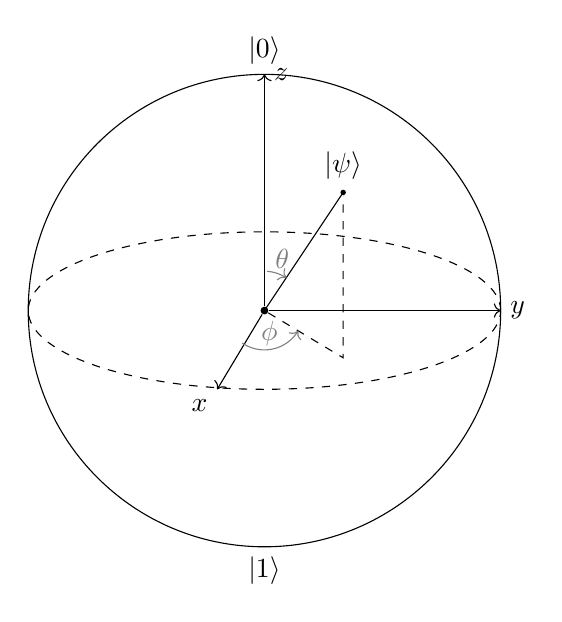
\begin{tikzpicture}

  % Define radius
  \def\r{3}

  % Bloch vector
  \draw (0,0) node[circle, fill, inner sep=1] (orig) {} -- (\r/3,\r/2)
    node[circle, fill, inner sep=0.7, label=above:$|\psi\rangle$] (psi) {};
  \draw[dashed] (orig) -- (\r/3, -\r/5) node (phi) {} -- (psi);

  % Sphere
  \draw (orig) circle (\r);
  \draw[dashed] (orig) ellipse (\r{} and \r/3);

  % Axes
  \draw[->] (orig) -- ++(-\r/5, -\r/3) node[below left] (x1) {$x$};
  \draw[->] (orig) -- ++(\r, 0) node[right] (x2) {$y$};
  \draw[->] (orig) -- ++(0, \r) node[right] (x3) {$z$};

  % Pole labels
  \node[above] at (0, \r) {$|0\rangle$};
  \node[below] at (0, -\r) {$|1\rangle$};

  % Angles
  \pic [draw=gray, text=gray, ->, "$\phi$"] {angle = x1--orig--phi};
  \pic [draw=gray, text=gray, <-, "$\theta$", angle eccentricity=1.4] {angle = psi--orig--x3};

\end{tikzpicture}
\caption{Bloch sphere representation of a qubit. The state $|\psi\rangle$ is represented as a point on the surface of a unit sphere, parameterized by angles $\theta$ and $\phi$.}
\label{fig:bloch}
\end{figure}


\textbf{Information content:} While the Bloch sphere has infinitely many points (suggesting infinite information storage), measurement reveals only a single classical bit. The continuous parameters $\alpha$ and $\beta$ can only be determined from infinitely many measurements of identically prepared qubits. Nature appears to keep track of this ``hidden information'' during quantum evolution, and this hidden quantum information grows exponentially with the number of qubits.

\subsection{Quantum gates}
Quantum gates are unitary operations that manipulate qubit states. Unlike classical gates, quantum gates are \textbf{reversible}—given the output and the gate operation, the input can always be determined. This reversibility is expressed mathematically by the unitarity constraint: for a gate represented by matrix $U$, we have $U^\dagger U = I$, where $U^\dagger$ is the conjugate transpose and $I$ is the identity matrix \cite{nielsen2011quantum, scherer2019mathematics}.

\textbf{Single-qubit gates:}

The quantum gates act linearly on superposition states. For example, if we define the Pauli-X (or simply X) gate by its action on basis states, it automatically defines its action on superpositions: $X(\alpha|0\rangle + \beta|1\rangle) = \alpha|1\rangle + \beta|0\rangle$.

\textit{Pauli-X gate:} The quantum analog of the NOT gate, with matrix representation:
\begin{equation}
X = \begin{pmatrix} 0 & 1 \\ 1 & 0 \end{pmatrix}
\end{equation}
It flips $|0\rangle$ to $|1\rangle$ and vice versa.

\textit{Pauli-Z gate:} Leaves $|0\rangle$ unchanged but flips the sign of $|1\rangle$:
\begin{equation}
Z = \begin{pmatrix} 1 & 0 \\ 0 & -1 \end{pmatrix}
\end{equation}

\textit{Hadamard gate (H):} Creates equal superposition and is crucial for quantum algorithms:
\begin{equation}
H = \frac{1}{\sqrt{2}}\begin{pmatrix} 1 & 1 \\ 1 & -1 \end{pmatrix}
\end{equation}
It transforms: $H|0\rangle = \frac{1}{\sqrt{2}}(|0\rangle + |1\rangle) = |+\rangle$ and $H|1\rangle = \frac{1}{\sqrt{2}}(|0\rangle - |1\rangle) = |-\rangle$. The Hadamard gate is sometimes described as a ``square-root of NOT'' gate. Notably, $H^2 = I$, so applying H twice returns the original state.

On the Bloch sphere, single-qubit gates correspond to rotations and reflections. The Hadamard operation is a rotation about the $\hat{y}$ axis by 90°, followed by a rotation about the $\hat{x}$ axis by 180°.

\textit{Phase gates (S, T):} Apply phase shifts to the $|1\rangle$ component.

\textit{Rotation gates:} $R_x(\theta)$, $R_y(\theta)$, $R_z(\theta)$ perform rotations around respective axes on the Bloch sphere by angle $\theta$.

\textbf{Two-qubit gates:}

\textit{CNOT (Controlled-NOT):} The prototypical multi-qubit gate, with two input qubits: a control and a target. It flips the target qubit if and only if the control qubit is $|1\rangle$. The transformation is:
\begin{align}
|00\rangle &\to |00\rangle \nonumber \\
|01\rangle &\to |01\rangle \nonumber \\
|10\rangle &\to |11\rangle \nonumber \\
|11\rangle &\to |10\rangle
\end{align}

This can be summarized as $|A,B\rangle \to |A, B \oplus A\rangle$, where $\oplus$ is addition modulo 2 (XOR). The matrix representation is:
\begin{equation}
\text{CNOT} = \begin{pmatrix} 
1 & 0 & 0 & 0 \\
0 & 1 & 0 & 0 \\
0 & 0 & 0 & 1 \\
0 & 0 & 1 & 0
\end{pmatrix}
\end{equation}

\begin{figure}[h]
\centering
\begin{quantikz}
\lstick{Control} & \ctrl{1} & \qw \\
\lstick{Target} & \targ{} & \qw
\end{quantikz}
\caption{Circuit diagram for the CNOT gate. The control qubit is on top with a filled circle, and the target qubit is below with the $\oplus$ symbol.}
\label{fig:cnot}
\end{figure}

\textit{CZ (Controlled-Z):} Applies a phase flip to the target qubit if the control is $|1\rangle$.

\textit{Controlled-U gates:} More generally, for any unitary $U$ acting on $n$ qubits, we can define a controlled-U gate with one control qubit. If the control is $|0\rangle$, nothing happens; if it's $|1\rangle$, $U$ is applied to the target qubits.

\textbf{Universality:} A fundamental result in quantum computing is that \textbf{any multiple qubit logic gate may be composed from CNOT and single-qubit gates}. This is the quantum analog of the universality of the NAND gate in classical computing. In fact, we only need certain specific single-qubit rotations (not arbitrary angles) to achieve universal quantum computation—we can build arbitrarily good approximations to any quantum gate using a finite set of fixed gates \cite{nielsen2011quantum}. Detailed proofs of universality and a complete treatment of single- and multi-qubit gates appear in Chapter~4 of~\cite{nielsen2011quantum}; Chapter~4 of~\cite{yanofsky2008quantum} provides a complementary exposition.

\textbf{No-Cloning Theorem:} Unlike classical bits, qubits cannot be copied. It is impossible to create a quantum circuit that takes an unknown quantum state $|\psi\rangle$ and produces two copies $|\psi\rangle|\psi\rangle$. This can be seen by attempting to use a CNOT gate for copying: applying CNOT to $(\alpha|0\rangle + \beta|1\rangle)|0\rangle$ yields $\alpha|00\rangle + \beta|11\rangle$, which is not equal to $|\psi\rangle|\psi\rangle = \alpha^2|00\rangle + \alpha\beta|01\rangle + \alpha\beta|10\rangle + \beta^2|11\rangle$ unless $\alpha\beta = 0$. This fundamental limitation has profound implications for quantum information processing \cite{nielsen2011quantum, yanofsky2008quantum}.

\textbf{No-Deleting Theorem:} Just as quantum information cannot be copied, it also cannot be destroyed. Closed quantum evolution is represented by unitary operators (which have an inverse) and therefore reversible: information about initial states is always preserved in the global system. No quantum operation can take two identical copies $|\psi\rangle|\psi\rangle$ and erase one to produce $|\psi\rangle|0\rangle$ for an arbitrary unknown state $|\psi\rangle$. This is the time-reversal dual of the no-cloning theorem, and both follow from the same underlying constraint—unitarity forbids the irreversible loss of information in an isolated quantum system.

\subsection{Quantum circuit}
A quantum circuit is a sequence of quantum gates applied to a set of qubits, analogous to classical circuits but with crucial differences \cite{nielsen2011quantum, johnston2019programming}. Quantum circuits are represented by circuit diagrams where:
\begin{itemize}
    \item Horizontal lines represent qubit wires (time flows left to right):
    \begin{center}
    \begin{quantikz}
        \lstick{$|q\rangle$} & \qw & \qw & \qw
    \end{quantikz}
    \end{center}

    \item Boxes or symbols represent quantum gates:
    \begin{center}
    \begin{quantikz}
        \lstick{$|q\rangle$} & \gate{H} & \gate{X} & \qw
    \end{quantikz}
    \end{center}

    \item Double lines represent classical bits (measurement outcomes):
    \begin{center}
    \begin{quantikz}
        \lstick{$c$} & \cw & \cw & \cw
    \end{quantikz}
    \end{center}

    \item Measurement is represented by a meter symbol:
    \begin{center}
    \begin{quantikz}
        \lstick{$|q\rangle$} & \qw & \meter{}
    \end{quantikz}
    \end{center}
\end{itemize}

Quantum circuits must:
\begin{enumerate}
    \item Initialize qubits in a known state (typically $|0\rangle$)
    \item Apply a sequence of unitary quantum gates
    \item Perform measurements to extract classical information
\end{enumerate}

Quantum circuits are \textbf{read from left to right}. The state of an $n$-qubit system is described by a vector in a $2^n$-dimensional Hilbert space. After applying gates $U_1, U_2, \ldots, U_m$ to an initial state $|\psi_0\rangle$, the final state is:
\begin{equation}
|\psi_f\rangle = U_m \cdots U_2 U_1 |\psi_0\rangle
\end{equation}

\begin{figure}[h]
\centering
\begin{quantikz}
    \lstick{$|\psi_0\rangle$} & \gate{U_1} & \gate{U_2} & \ \ldots\ & \gate{U_m} & \rstick{$|\psi_f\rangle$} \qw
\end{quantikz}
\caption{A generic quantum circuit applying gates $U_1, U_2, \ldots, U_m$ in sequence to an initial state $|\psi_0\rangle$, producing the final state $|\psi_f\rangle = U_m \cdots U_1 |\psi_0\rangle$. Gates are applied left to right, but compose right to left in matrix notation.}
\label{fig:generic_circuit}
\end{figure}

\textbf{Differences from classical circuits:}
\begin{itemize}
    \item Quantum circuits are \textbf{acyclic}—no feedback loops are allowed
    \item No FANIN operation (joining wires), as this is not reversible
    \item No FANOUT operation (copying qubits), due to the no-cloning theorem
    \item All operations except measurement are reversible (unitary)
\end{itemize}

\textbf{Example: SWAP circuit}
A useful quantum circuit swaps the states of two qubits using three CNOT gates:

\begin{figure}[h]
\centering
\begin{quantikz}
\lstick{$|a\rangle$} & \ctrl{1} & \targ{} & \ctrl{1} & \qw & \rstick{$|b\rangle$} \\
\lstick{$|b\rangle$} & \targ{} & \ctrl{-1} & \targ{} & \qw & \rstick{$|a\rangle$}
\end{quantikz}
\caption{SWAP circuit using three CNOT gates to exchange the states of two qubits.}
\label{fig:swap}
\end{figure}

The operation can be verified: $|a,b\rangle \to |a, a\oplus b\rangle \to |a \oplus (a\oplus b), a\oplus b\rangle = |b, a\oplus b\rangle \to |b, (a\oplus b) \oplus b\rangle = |b,a\rangle$.

\textbf{Multiple Qubits:}
For $n$ qubits, the computational basis states are of the form $|x_1x_2\ldots x_n\rangle$, and a quantum state is specified by $2^n$ complex amplitudes. For $n=500$, this number exceeds the estimated number of atoms in the Universe! This exponential scaling represents enormous potential computational power, as Nature appears to manipulate such quantities during quantum evolution.


\subsection{Bell states}
Bell states (also called EPR pairs, after Einstein, Podolsky, and Rosen) are maximally entangled two-qubit states that exhibit remarkable quantum correlations \cite{nielsen2011quantum}. The four Bell states are:

\begin{align}
|\beta_{00}\rangle &= \frac{|00\rangle + |11\rangle}{\sqrt{2}} \\
|\beta_{01}\rangle &= \frac{|01\rangle + |10\rangle}{\sqrt{2}} \\
|\beta_{10}\rangle &= \frac{|00\rangle - |11\rangle}{\sqrt{2}} \\
|\beta_{11}\rangle &= \frac{|01\rangle - |10\rangle}{\sqrt{2}}
\end{align}

These states can be generated using a simple quantum circuit consisting of a Hadamard gate followed by a CNOT gate:

\begin{figure}[h]
\centering
\begin{quantikz}
\lstick{$|0\rangle$} & \gate{H} & \ctrl{1} & \qw & \rstick{$\frac{|00\rangle + |11\rangle}{\sqrt{2}}$} \\
\lstick{$|0\rangle$} & \qw & \targ{} & \qw & 
\end{quantikz}
\caption{Circuit for generating the Bell state $|\beta_{00}\rangle$. The Hadamard gate creates superposition, and the CNOT entangles the qubits.}
\label{fig:bell_circuit}
\end{figure}

\textbf{Properties and significance:}
\begin{itemize}
    \item \textbf{Entanglement:} Measuring one qubit instantly determines the measurement outcome of the other, regardless of spatial separation
    \item \textbf{Non-classical correlations:} John Bell proved that measurement correlations in Bell states are stronger than could ever exist between classical systems
    \item \textbf{Quantum teleportation:} Bell states are the key resource for quantum teleportation, allowing quantum information to be transmitted using only classical communication and pre-shared entanglement
    \item \textbf{Superdense coding:} Bell states enable sending two classical bits using only one qubit
    \item \textbf{Quantum cryptography:} Used in quantum key distribution protocols
\end{itemize}

When measuring the first qubit of $|\beta_{00}\rangle$, we obtain:
\begin{itemize}
    \item Result 0 with probability 1/2, leaving post-measurement state $|00\rangle$
    \item Result 1 with probability 1/2, leaving post-measurement state $|11\rangle$
\end{itemize}

Thus, measurement outcomes are perfectly correlated—if the first qubit measures 0, the second must also measure 0, and similarly for 1. These correlations persist for other types of measurements and cannot be explained by classical hidden variables. For a comprehensive treatment of quantum entanglement, the EPR argument, and Bell inequalities, we refer to Chapter~2 of~\cite{nielsen2011quantum} and Chapter~7 of~\cite{yanofsky2008quantum}.


\subsection{Pauli matrices}
The Pauli matrices are a set of three $2 \times 2$ complex Hermitian matrices that form a basis for the space of $2 \times 2$ Hermitian matrices (along with the identity matrix). They are fundamental operators in quantum mechanics and quantum computing \cite{nielsen2011quantum, scherer2019mathematics}.

The three Pauli matrices are:
\begin{equation}
\sigma_x = X = \begin{pmatrix} 0 & 1 \\ 1 & 0 \end{pmatrix}, \quad
\sigma_y = Y = \begin{pmatrix} 0 & -i \\ i & 0 \end{pmatrix}, \quad
\sigma_z = Z = \begin{pmatrix} 1 & 0 \\ 0 & -1 \end{pmatrix}
\end{equation}

Key properties:
\begin{itemize}
\item They are Hermitian: $\sigma_i^\dagger = \sigma_i$
\item They are unitary: $\sigma_i^2 = I$ (the identity matrix)
\item They satisfy anticommutation relations: $\{\sigma_i, \sigma_j\} = 2\delta_{ij}I$
\item They satisfy commutation relations: $[\sigma_i, \sigma_j] = 2i\epsilon_{ijk}\sigma_k$
\item They are traceless: $\text{Tr}(\sigma_i) = 0$
\end{itemize}

\textbf{Pauli strings for multi-qubit systems:}
For multi-qubit systems, Pauli strings are formed by tensor products of single-qubit Pauli operators. For example, for a three-qubit system: $X \otimes Z \otimes I$, which applies X to the first qubit, Z to the second, and identity (nothing) to the third.

\begin{figure}[h]
\centering
\begin{quantikz}
    \lstick{$|q_1\rangle$} & \gate{X} & \qw \\
    \lstick{$|q_2\rangle$} & \gate{Z} & \qw \\
    \lstick{$|q_3\rangle$} & \qw      & \qw
\end{quantikz}
\caption{Circuit representation of the Pauli string $X \otimes Z \otimes I$. An $X$ gate acts on qubit 1, a $Z$ gate acts on qubit 2, and qubit 3 passes through unchanged (identity).}
\label{fig:pauli_string}
\end{figure}

These Pauli strings form a complete basis for decomposing arbitrary operators on $n$ qubits. Any $2^n \times 2^n$ matrix can be written as a linear combination of $4^n$ Pauli strings (including identity). This decomposition is crucial for quantum algorithms.

\textbf{Relevance to VQLS:}
In the context of VQLS, the number of Pauli terms in the decomposition of the system matrix directly impacts:
\begin{itemize}
    \item Circuit complexity (more terms require more measurements)
    \item Measurement overhead (each Pauli string requires separate measurement circuits)
    \item Overall algorithm efficiency
\end{itemize}

Reducing the number of Pauli terms is therefore a key optimization target for VQLS implementations. The algebraic properties of the Pauli matrices and their use as an operator basis are developed in detail in Chapter~1 of~\cite{nielsen2011quantum} and Chapter~3 of~\cite{scherer2019mathematics}.

\subsection{VQLS}
Variational Quantum Linear Solver (VQLS) is a quantum algorithm designed to solve linear systems of equations $A|\mathbf{x}\rangle = |\mathbf{b}\rangle$ on near-term quantum devices \cite{bravo2023vqls}. Unlike the HHL algorithm, VQLS is a hybrid quantum-classical algorithm suitable for NISQ devices.

\textbf{Analogy with machine learning.}
VQLS is structurally very similar to supervised machine learning. In both cases:
\begin{itemize}
    \item A \textit{model with trainable parameters} $\boldsymbol{\theta}$ is defined (a neural network in ML; a parameterized quantum circuit in VQLS).
    \item A \textit{loss function} measures how far the current parameters are from the desired output.
    \item A \textit{classical optimizer} (e.g.\ gradient descent) iteratively updates $\boldsymbol{\theta}$ to minimize the loss.
    \item Training \textit{converges} when the loss is sufficiently small.
\end{itemize}
The key difference is that in VQLS the model lives on a quantum computer: the ``forward pass'' is a quantum circuit measurement, and the expressivity of the model comes from quantum superposition and entanglement rather than from the depth of a neural network \cite{schuld2018supervised, wittek2014quantum}.

The VQLS algorithm works by:

1. \textbf{Ansatz preparation:} Preparing a parameterized quantum state $\ket{\psi(\boldsymbol{\theta})} = V(\boldsymbol{\theta})\ket{0}$ using a variational quantum circuit. A common choice is the hardware-efficient ansatz (see Figure \ref{fig:ansatz}).

\textit{Ansatz analogy.} The word \textit{ansatz} (German for ``initial guess'' or ``approach'') refers to a family of quantum states parameterized by angles $\boldsymbol{\theta}$. Think of it like a function template: just as a data scientist might choose a neural network architecture (how many layers, what activations) before training, a quantum engineer chooses an ansatz circuit structure. The parameters $\boldsymbol{\theta}$ are then adjusted during training to find the best approximation to the solution of the linear system. The choice of ansatz is crucial: it must be expressive enough to capture the solution but also efficient enough to run on NISQ hardware.


\begin{figure}[h]
\centering
\begin{quantikz}
\lstick{$\ket{0}$} & \gate{R_y(\theta_1)} & \ctrl{1} & \qw      & \gate{R_y(\theta_4)} & \qw \\
\lstick{$\ket{0}$} & \gate{R_y(\theta_2)} & \targ{}  & \ctrl{1} & \gate{R_y(\theta_5)} & \qw \\
\lstick{$\ket{0}$} & \gate{R_y(\theta_3)} & \qw      & \targ{}  & \gate{R_y(\theta_6)} & \qw
\end{quantikz}
\caption{Example of a 3-qubit Hardware-Efficient Ansatz. $R_y$ gates provide trainable rotations, while CNOTs provide entanglement.}
\label{fig:ansatz}
\end{figure}

2. \textbf{Cost function:} Defining a cost function that measures how well $A\ket{\psi(\boldsymbol{\theta})}$ aligns with $\ket{b}$. This often involves the Hadamard Test (Figure \ref{fig:hadamard_test}) to compute the terms $\langle b|A|\psi(\boldsymbol{\theta})\rangle$.



\begin{figure}[h]
\centering
\begin{quantikz}
\lstick{Ancilla $\ket{0}$} & \gate{H} & \ctrl{1} & \gate{H} & \meter{} \\
\lstick{System $\ket{\psi}$} & \qw      & \gate{U} & \qw      & \qw      
\end{quantikz}
\caption{The Hadamard Test circuit used to evaluate overlaps. In VQLS, $U$ is replaced by operations related to $A$ and the state preparation of $b$.}
\label{fig:hadamard_test}
\end{figure}

3. \textbf{Classical optimization:} Using a classical optimizer (like gradient descent) to adjust $\boldsymbol{\theta}$ to minimize $C(\boldsymbol{\theta})$.

4. \textbf{Measurement:} Evaluating expectation values through quantum measurements.

\textbf{Pauli decomposition and efficiency:}
The computational cost of VQLS depends heavily on how the matrix $A$ is decomposed into Pauli strings:
\begin{equation}
A = \sum_{i=1}^{M} c_i P_i
\end{equation}
Each Pauli term requires separate measurement circuits, so minimizing $M$ is crucial for efficiency. This is where discretization methods become important.

\subsection{ODE type}
Ordinary Differential Equations (ODEs) are equations involving functions and their derivatives. Many scientific and engineering problems can be formulated as ODEs \cite{scherer2019mathematics, woody2022essential}. A general form of an ODE is:
\begin{equation}
\frac{dy}{dt} = f(t, y)
\end{equation}
where $y$ is the unknown function and $f$ is a known function.

Linear ODEs are particularly important and can be written as:
\begin{equation}
\frac{dy}{dt} + p(t)y = q(t)
\end{equation}

When discretized, ODEs can be converted into linear systems of equations. Different discretization methods (finite difference, finite element, spectral methods) lead to different matrix structures. For quantum linear solvers, the choice of discretization method affects:
\begin{itemize}
\item The sparsity pattern of the resulting matrix
\item The condition number of the system
\item The number of Pauli terms needed for quantum representation
\item The overall quantum circuit depth and complexity
\end{itemize}

\textbf{Example - Second-order ODE (Poisson equation):}
Consider the boundary value problem:
\begin{equation}
-\frac{d^2u}{dx^2} = f(x), \quad u(0) = u(1) = 0
\end{equation}
This is the one-dimensional Poisson equation, a canonical PDE benchmark in quantum computing research \cite{mukhanbet2024poisson}. Finite difference discretization with $n$ grid points yields a tridiagonal matrix, while spectral methods using Chebyshev or Legendre polynomials produce dense but structured matrices \cite{childs2020spectral}. Understanding which approach leads to fewer Pauli terms is the central question of this research.

\subsection{Spectral methods}
Spectral methods are a class of numerical techniques for solving differential equations that represent the solution as a sum of basis functions (typically orthogonal polynomials or Fourier modes). Unlike finite difference or finite element methods that provide pointwise approximations, spectral methods approximate the global behavior of the solution \cite{scherer2019mathematics}.

Common spectral bases include:
\begin{itemize}
\item \textbf{Fourier series:} For periodic problems on regular domains
\begin{equation}
u(x) = \sum_{k=-N}^{N} \hat{u}_k e^{ikx}
\end{equation}

\item \textbf{Chebyshev polynomials:} For non-periodic problems on bounded intervals $[-1,1]$
\begin{equation}
u(x) = \sum_{k=0}^{N} \hat{u}_k T_k(x)
\end{equation}
where $T_k(x) = \cos(k \arccos(x))$

\item \textbf{Legendre polynomials:} For problems on $[-1, 1]$ with natural boundary conditions
\begin{equation}
u(x) = \sum_{k=0}^{N} \hat{u}_k P_k(x)
\end{equation}
\end{itemize}

The key advantages of spectral methods are:
\begin{itemize}
\item \textbf{Exponential convergence} for smooth solutions (spectral accuracy)
\item High accuracy with fewer degrees of freedom compared to finite differences
\item Dense but structured matrices with special mathematical properties
\item Well-understood conditioning and stability properties
\end{itemize}

\textbf{Disadvantages:}
\begin{itemize}
\item Dense matrices (though structured)
\item Less flexible for complex geometries
\item Reduced accuracy for non-smooth solutions
\end{itemize}

\textbf{Connection to VQLS:}
In the context of VQLS, spectral methods produce matrices with specific structures that may decompose into fewer Pauli terms compared to standard finite difference discretizations. The dense but structured nature of spectral matrices could potentially be exploited for more efficient Pauli decompositions, reducing quantum circuit complexity. This hypothesis is motivated by the work of Childs and Liu~\cite{childs2020spectral}, who showed that spectral discretizations yield quantum algorithms for ODEs with complexity poly$(\log d,\, \log(1/\epsilon))$ — exponentially better in the error $\epsilon$ than finite-difference-based approaches. This hypothesis forms the core of our research question.

\subsection{Simulation vs Quantum}
Classical simulation of quantum circuits is possible but becomes exponentially expensive as the number of qubits increases. A classical computer must track $2^n$ complex amplitudes for an $n$-qubit system, making exact simulation intractable for systems with more than approximately 50 qubits \cite{nielsen2011quantum, hidary2021quantum}.

However, for small-scale problems, classical simulation is valuable for:
\begin{itemize}
\item Algorithm development and testing
\item Verification of quantum results
\item Benchmarking quantum advantage
\item Understanding noise effects
\item Debugging quantum circuits before running on expensive hardware
\end{itemize}

The transition from simulation to actual quantum hardware introduces challenges:
\begin{itemize}
\item \textbf{Noise and errors:} Real quantum devices suffer from decoherence and gate errors
\item \textbf{Limited connectivity:} Qubits may not all be directly connected, requiring SWAP gates
\item \textbf{Measurement limitations:} Statistical sampling is needed to estimate expectation values
\item \textbf{Calibration:} Gate fidelities vary and require regular calibration
\item \textbf{Coherence time:} Limited time before quantum information is lost
\end{itemize}

For this project, classical simulation allows us to investigate whether spectral methods reduce Pauli term counts in a controlled environment before considering implementation on actual quantum hardware. The simulation results will inform whether the approach is promising enough to warrant the complexity and cost of real quantum execution.

\section{Problem statement}
Standard discretization methods for differential equations, such as finite difference schemes, often produce sparse matrices when converted to quantum representations. However, these matrices may decompose into a large number of Pauli terms, which increases the measurement overhead and circuit complexity for variational quantum linear solvers.

Spectral methods offer an alternative discretization approach that produces different matrix structures—typically denser but with specific mathematical properties. The central question of this research is: \textbf{Can spectral methods reduce the number of Pauli terms needed to represent discretized differential operators in VQLS, thereby improving the efficiency of quantum linear solving algorithms?}

More specifically, we investigate:
\begin{enumerate}
\item How does the Pauli term count compare between spectral methods and finite difference methods for common differential operators?
\item Does the structured nature of spectral method matrices lead to more efficient Pauli decompositions?
\item What is the trade-off between matrix density and Pauli term count?
\item How does this affect the overall quantum circuit depth and measurement requirements for VQLS?
\item Does the exponential convergence of spectral methods provide any advantage in the quantum setting?
\end{enumerate}

Understanding this relationship could lead to significant improvements in VQLS implementations for solving differential equations, which have applications across scientific computing, fluid dynamics, quantum chemistry, and machine learning.

\section{Results}

This section presents four experiments that progressively characterize the Pauli structure of spectral collocation matrices. The central tool is the \emph{basis-change identity}: for any polynomial basis $\{\phi_j\}$ with lower-triangular coefficient matrix $C$ (so $\phi_j(t) = \sum_{k=0}^{j} C_{jk}\,t^k$), the collocation matrix satisfies
\begin{equation}
    M = A_{\mathrm{mono}}\,C^{\top},
\end{equation}
where $A_{\mathrm{mono}}$ is the collocation matrix for the monomial basis $\phi_j(t)=t^j$. Since $C$ is invertible whenever the basis is non-degenerate, every non-singular collocation matrix $M$ is reachable by an appropriate basis choice, and the Pauli count becomes a property of $M$ alone, independent of how $C$ is parameterized.

\subsection{Experiment 1: Second-order ODE with pure second derivative}

\paragraph{Setup.}
We consider the boundary value problem
\begin{equation}
    u''(t) = 0, \qquad t \in [0,1], \qquad u(0) = 0,\quad u(1) = 1,
\end{equation}
with interior collocation requirements $u''(1/3) = 0$ and $u''(2/3) = 0$. Using a degree-3 trial function $u(t) = \sum_{j=0}^{3} a_j\phi_j(t)$, these four conditions yield a $4 \times 4$ collocation matrix ($N=4$, two qubits).

\paragraph{Case A: Monomial basis.}
With $\phi_j(t) = t^j$, the system matrix is
\begin{equation}
A_{\mathrm{mono}} =
\begin{bmatrix}
1 & 0 & 0 & 0 \\
1 & 1 & 1 & 1 \\
0 & 0 & 2 & 2 \\
0 & 0 & 2 & 4
\end{bmatrix},
\end{equation}
which requires all 16 two-qubit Pauli strings.

\paragraph{Case B: Block-diagonal analytical construction.}
The operator $L[\cdot] = (\cdot)''$ annihilates every polynomial of degree $\leq 1$, so the collocation rows automatically contain zeros in the first two columns for any basis choice. Exploiting this lower-left zero block, we impose three structural conditions on $C$ to also zero the upper-right block:
\begin{enumerate}
    \item $C_{20}=0$, $C_{30}=0$, $C_{21}+C_{22}=0$, $C_{31}+C_{32}+C_{33}=0$ (upper-right block = 0),
    \item $B_1 = B_2$ (equal diagonal blocks, eliminating $Z \otimes \cdot$ Pauli strings),
    \item $C_{10} = C_{00}$ (repeated first-column entry, eliminating $IY$).
\end{enumerate}
With the concrete choice $C_{00}=2$, $C_{11}=2$, $C_{10}=2$, $C_{22}=1$, $C_{21}=-1$, $C_{33}=1$, $C_{32}=0$, $C_{31}=-1$, the collocation matrix becomes
\begin{equation}
A =
\begin{bmatrix}
2 & 2 & 0 & 0 \\
2 & 4 & 0 & 0 \\
0 & 0 & 2 & 2 \\
0 & 0 & 2 & 4
\end{bmatrix},
\end{equation}
and its (normalized) Pauli decomposition is
\begin{equation}
    \frac{A}{\|A\|} \approx 0.4009\,II + 0.2673\,IX - 0.1336\,IZ,
\end{equation}
an \textbf{81\% reduction} from 16 to 3 Pauli strings.

\paragraph{Why three is the minimum in the block-diagonal family.}
With a $2\times 2$ block $B = \bigl[\begin{smallmatrix}a&a\\a&c\end{smallmatrix}\bigr]$, the surviving Pauli coefficients are $\alpha=(a+c)/2$, $\beta=a$, $\gamma=(a-c)/2$. Eliminating $IZ$ would require $a=c$, making $\det(B)=0$; the system would have no unique solution. Hence three Pauli strings is the minimum within the block-diagonal family.

\paragraph{Global LP.}
By the basis-change identity, minimizing $\sum_P |c_P(M)|$ subject to $\operatorname{Tr}(M)=4$ over all entries of $M$ is a linear program. The HiGHS simplex solver finds the global optimum $M^* = I_4$, with a single Pauli string ($c_{II}=1$, all others zero) --- a \textbf{94\% reduction} from Case~A. The corresponding dual basis is
\begin{align*}
    \phi_0(t) &= 1 - t, \\
    \phi_1(t) &= t, \\
    \phi_2(t) &= -\tfrac{1}{2}t + t^2 - \tfrac{1}{2}t^3, \\
    \phi_3(t) &= -\tfrac{1}{2}t^2 + \tfrac{1}{2}t^3,
\end{align*}
with $\det C = \tfrac{1}{4} \neq 0$. Solving $I_4\,\mathbf{a}=\mathbf{b}$ gives $\mathbf{a}=\mathbf{b}=[0,1,0,0]^\top$, recovering the exact solution $u(t) = t$.

\begin{center}
\begin{tabular}{lcc}
\hline
Basis & Pauli strings & Reduction \\
\hline
Case A (monomial)              & 16/16 & --- \\
Case B (block-diagonal, monic) &  3/16 & 81\% \\
LP global optimum ($M^*=I_4$)  &  1/16 & 94\% \\
\hline
\end{tabular}
\end{center}

\subsection{Experiment 2: ODE with lower-order terms}

\paragraph{Setup.}
We now consider the full second-order problem
\begin{equation}
    u''(t) + u'(t) + u(t) = t^2 + 3t + 3, \qquad t \in [-1,1], \qquad u(-1)=0,\quad u(1)=2,
\end{equation}
with collocation requirements $L[u](\pm 1/3) = f(\pm 1/3)$. The exact solution is $u(t) = t^2 + t$.

\paragraph{Obstruction to block-diagonal structure.}
Unlike Experiment~1, the identity term in $L[\cdot] = (\cdot)'' + (\cdot)' + (\cdot)$ gives $L[\phi_0] = C_{00} \neq 0$ and couples the collocation rows to the lower-degree basis functions. Forcing the lower-left $2\times 2$ block to zero requires $C_{00}=0$, $C_{11}=0$, $C_{10}=0$, which degenerates the basis. The block-diagonal strategy from Experiment~1 is \emph{structurally impossible} when the differential operator contains lower-order terms.

\paragraph{Global LP.}
Despite this obstruction, the LP over all entries of $M$ is unaffected: it finds the same global optimum $M^* = I_4$, with a single Pauli string. The corresponding dual basis has operator-dependent coefficients (e.g.\ $\phi_0(t) \approx 0.4525 - 0.5792t + 0.0475t^2 + 0.0792t^3$), but the quantum representation is identical to Experiment~1. Solving $I_4\,\mathbf{a}=\mathbf{b}$ recovers the exact solution $u(t)=t^2+t$ at all test points.

\paragraph{Key implication.}
The Pauli count of the collocation matrix is \emph{independent of the differential operator}. For any second-order ODE on any domain with two boundary conditions and two interior collocation points, the globally optimal collocation matrix is $M^*=I_4$, achieved by a suitably chosen operator-dependent dual basis.

\begin{center}
\begin{tabular}{lcc}
\hline
Basis & Pauli strings & Reduction \\
\hline
Case A (monomial)             & 16/16 & --- \\
LP global optimum ($M^*=I_4$) &  1/16 & 94\% \\
\hline
\end{tabular}
\end{center}

\subsection{Experiment 3: Scaling to three qubits}

\paragraph{Setup.}
We return to the Experiment~2 ODE but scale to $N=8$ (three qubits): two boundary rows and \textbf{six} interior collocation rows at equidistant points $t_k = -1 + k/7$ for $k=1,\ldots,6$, with a degree-7 polynomial trial function.

\paragraph{Case A.}
The monomial collocation matrix $A_{\mathrm{mono}}$ is $8\times 8$ with $\det A_{\mathrm{mono}} \approx 1003.4$, non-singular. It decomposes into all $4^3 = \mathbf{64}$ three-qubit Pauli strings. Adding more collocation points does not improve the Pauli structure---it only makes it exponentially worse.

\paragraph{Global LP.}
The LP over all $64$ entries of $M$ (with $\operatorname{Tr}(M)=8$) again finds $M^* = I_8$, with a single Pauli string $c_{III}=1$ --- a \textbf{98.4\% reduction}. The dual basis $\phi_0,\ldots,\phi_7$ is verified numerically at five test points, recovering $u(t)=t^2+t$ to machine precision.

\paragraph{Universal pattern.}
Across all three experiments the LP always returns $M^*=I_N$:

\begin{center}
\begin{tabular}{ccccc}
\hline
Experiment & $N$ & Qubits & Case A & LP optimum \\
\hline
1 & 4 & 2 & 16/16 & 1/16 \\
2 & 4 & 2 & 16/16 & 1/16 \\
3 & 8 & 3 & 64/64 & 1/64 \\
\hline
\end{tabular}
\end{center}

\paragraph{Why $M^*=I_N$ is always optimal.}
The identity matrix $I_N$ concentrates all its Pauli weight into the identity string $I^{\otimes n}$. Formally, $c_{I\cdots I}(I_N)=1$ and $c_P(I_N)=\operatorname{Tr}(P)/N=0$ for all non-identity $P$, since every non-identity Pauli string is traceless. No other matrix achieves fewer Pauli strings subject to $\operatorname{Tr}(M)=N$.

\paragraph{VQLS implication.}
With $M^*=I_N$, the VQLS system reduces to $I\ket{\psi}=\ket{b}$, which is trivially solved by $\ket{\psi}=\ket{b}$. This is classically trivial and does not provide a quantum advantage. The open question is whether there exists a non-trivial class of operators for which the LP optimum is greater than 1 but still polynomially small in $n$---the regime where VQLS could offer a genuine speedup.

\subsection{Experiment 4: Monic LP as a middle ground}

\paragraph{Motivation.}
Experiments 1--3 identified two extreme strategies: Case~A (all $4^n$ Pauli strings, no optimization) and the global LP (1 Pauli string, classically trivial). This raises the question: \emph{can we reduce the Pauli count substantially while keeping the quantum system non-trivial?}

\paragraph{Monic LP formulation.}
We restrict $C$ to be \emph{lower-triangular with unit diagonal} ($C_{jj}=1$, $C_{jk}=0$ for $k>j$, $C_{jk}$ free for $k<j$). This ``monic'' restriction fixes $\phi_j$ to be a degree-$j$ polynomial with leading coefficient~1. Writing $C = I + \Delta$ where $\Delta$ is strictly lower-triangular, the collocation matrix becomes $M = A_{\mathrm{mono}}(I+\Delta)^\top$, which is affine in the $\tfrac{N(N-1)}{2}$ free entries of $\Delta$. The resulting LP is
\begin{equation}
    \min_{\mathbf{x},\,\mathbf{t}}\;\sum_{P} t_P
    \qquad\text{s.t.}\quad J\mathbf{x} + \mathbf{c}^0 \leq \mathbf{t},\;
    -J\mathbf{x} - \mathbf{c}^0 \leq \mathbf{t},\;
    \mathbf{t} \geq 0,
\end{equation}
where $\mathbf{c}^0$ are the Case~A Pauli coefficients and $J$ is the Jacobian of $c_P$ with respect to $\Delta$. The unit-diagonal constraint ensures $C$ is always invertible, so no normalization constraint ($\operatorname{Tr}(M)=N$) is needed.

\paragraph{Results.}
Table~\ref{tab:monic} summarizes the Pauli counts and VQLS Hadamard-test overhead across all experiments.

\begin{table}[h]
\centering
\caption{Pauli strings and Hadamard tests per VQLS step (HT/step $= L^2(n+1)$) for each experiment and basis choice.}
\label{tab:monic}
\begin{tabular}{lccccc}
\hline
Experiment & $N$ & $n$ & Case A & Monic LP & Global LP \\
\hline
Exp.~1: $u''=0$ on $[0,1]$                    & 4 & 2 & 16/16 & \textbf{6/16}  & 1/16 \\
Exp.~2: $u''+u'+u=f$ on $[-1,1]$              & 4 & 2 & 16/16 & \textbf{10/16} & 1/16 \\
Exp.~3: $u''+u'+u=f$ on $[-1,1]$ (3 qubits)  & 8 & 3 & 64/64 & \textbf{36/64} & 1/64 \\
\hline
Exp.~1 HT/step & & & 768 & \textbf{108} & 3 \\
Exp.~2 HT/step & & & 768 & \textbf{300} & 3 \\
Exp.~3 HT/step & & & 16{,}384 & \textbf{5{,}184} & 4 \\
\hline
\end{tabular}
\end{table}

For Experiment~1, the monic LP returns the basis coefficient matrix
\begin{equation}
C^* =
\begin{bmatrix}
1 & 0 & 0 & 0 \\
\tfrac{1}{2} & 1 & 0 & 0 \\
0 & -1 & 1 & 0 \\
0 & \tfrac{1}{4} & -\tfrac{5}{4} & 1
\end{bmatrix},
\end{equation}
yielding six nonzero Pauli strings $\{II, IX, IY, ZI, ZY, ZZ\}$.

\paragraph{Why the monic LP cannot recover the 3-Pauli Case~B solution.}
The analytical block-diagonal strategy in Experiment~1 uses a non-unit diagonal (e.g.\ $C_{00}=C_{11}=2$). Normalizing to a unit diagonal changes the resulting $M$ and produces six nonzero Pauli strings---identical to the monic LP optimum. The 3-Pauli solution therefore lies outside the monic family; it requires non-unit diagonal scaling.

\paragraph{VQLS convergence.}
VQLS was run with a hardware-efficient $R_Y$-CNOT ansatz for 25 gradient steps (3 trials per configuration, seeds 0--2). For $N=4$ (Experiment~2 ODE), timing was measured on classical simulation. Table~\ref{tab:vqls_timing} reports the LP preprocessing time, VQLS wall-clock time per 25 steps, and final cost.

\begin{table}[h]
\centering
\caption{VQLS timing and convergence results for $N=4$ (Experiment~2 ODE, classical simulation, 25 steps, 3 trials). LP times are negligible ($\lesssim 0.13$\,s). VQLS wall-clock time scales with HT/step: the monomial basis requires $237\times$ more simulation time than the full LP.}
\label{tab:vqls_timing}
\begin{tabular}{lcccc}
\hline
Basis & Paulis & HT/step & VQLS time (s) & Cost @ 25 steps \\
\hline
Monomial (Case A) & 16 & 768   & $637 \pm 115$ & $0.185 \pm 0.000$ \\
Monic LP          & 10 & 300   & $220 \pm 15$  & $0.294 \pm 0.000$ \\
Full LP           &  1 & 3     & $2.7 \pm 0.7$ & $0.025 \pm 0.000$ \\
\hline
\end{tabular}
\end{table}

The LP preprocessing step (solving for the optimal basis) takes $0.13$\,s for the monic LP and $0.11$\,s for the full LP---negligible compared to VQLS runtime. VQLS wall-clock time scales closely with HT/step: the monic LP is $2.9\times$ faster than Case~A, and the full LP is $237\times$ faster. Despite this, final cost values do not monotonically improve: the cost plateaus at $0.025$--$0.29$ for all methods. This is an \emph{ansatz limitation}: the single-layer $R_Y$ circuit with $n$ parameters cannot express the exact solution state $\ket{b}$ for general $b$. Pauli overhead reduction speeds up each gradient step but does not expand ansatz expressivity.

\begin{figure}[h]
\centering
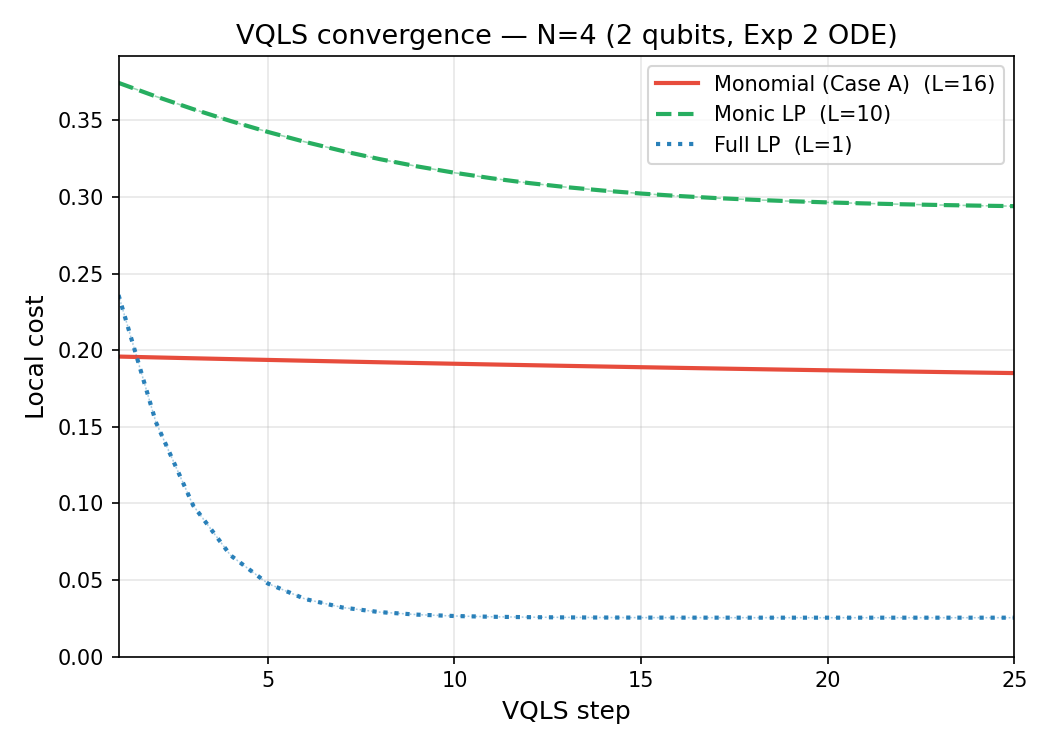
\includegraphics[width=0.75\textwidth]{../plots/scaling_N4.png}
\caption{VQLS convergence curves for $N=4$ (2 qubits) on the Experiment~2 ODE, comparing monomial (Case~A), monic LP, and full LP bases over 25 gradient steps. The full LP converges fastest due to minimal Hadamard-test overhead; the monic LP is intermediate. All three plateau due to the expressivity limit of the single-layer ansatz.}
\label{fig:vqls_convergence}
\end{figure}

\paragraph{Non-triviality.}
Crucially, the monic LP result $M^* \neq I_N$, so the VQLS system $M^*\ket{\psi}=\ket{b}$ is not classically trivial. Unlike the global LP, the monic LP does not collapse the quantum problem into a state-preparation task.

\paragraph{Structural simplicity.}
The monic LP is modestly simpler than the global LP: it has $\tfrac{N(N-1)}{2}$ free variables (vs.\ $N^2$ for the global LP) and requires no normalization constraint. Both are $O(N^2)$-variable LPs solved in milliseconds by HiGHS.

\section{Conclusion}

This paper studied whether the choice of polynomial basis in spectral collocation methods can reduce the Pauli term count of system matrices used in Variational Quantum Linear Solvers (VQLS). Through four experiments on second-order boundary value problems, we established the following findings.

\textbf{The monomial basis is the worst case.} The standard monomial (Case~A) basis saturates all $4^n$ available Pauli strings for any $n$-qubit collocation problem, regardless of the differential operator. This is the natural starting point but also the most expensive for VQLS.

\textbf{A basis-change identity reduces Pauli minimization to a linear program.} Any non-singular collocation matrix is reachable by an appropriate polynomial basis, so minimizing Pauli count over all basis choices is equivalent to a linear program over the collocation matrix $M$.

\textbf{The global LP always finds $M^*=I_N$.} The identity matrix is the unique LP optimum subject to $\operatorname{Tr}(M)=N$, achieving a single Pauli string regardless of the operator, domain, or boundary conditions. This represents a 94--98\% reduction in Pauli terms. However, $M^*=I_N$ collapses the quantum system to $I\ket{\psi}=\ket{b}$, which is classically trivial and offers no quantum advantage.

\textbf{The monic LP provides a principled middle ground.} By restricting the basis coefficient matrix to be lower-triangular with unit diagonal, the monic LP reduces Hadamard-test overhead by factors of $3$--$7\times$ across the three experimental settings while preserving a non-trivial quantum system ($M^* \neq I_N$). It is structurally simpler than the global LP (no normalization constraint) and naturally parameterized in terms of the polynomial basis.

\textbf{Ansatz expressivity is the binding bottleneck at small scales.} In the VQLS experiments, convergence quality is determined by the expressivity of the single-layer $R_Y$ ansatz, not by Pauli overhead. At $N=4,8$, any classical method trivially solves the problem, so no VQLS formulation at this scale offers a quantum advantage. The Pauli reductions identified here become meaningful only at much larger $N$, where quantum linear solvers are hypothesized to offer exponential advantages.

\textbf{Open problems.} The most important open question is whether there exists a non-trivial class of ODEs or boundary conditions for which the LP Pauli optimum is greater than 1 but still polynomially small in the number of qubits. Such a class would be a natural candidate for genuine near-term quantum advantage in differential equation solving. Extensions to higher-dimensional problems (PDEs), non-polynomial right-hand sides, and actual NISQ hardware experiments are left for future work.

\section{Appendix}

\subsection*{Code}
All code is publicly available at \url{https://github.com/proxy-pylon/math-499}.

The repository contains the following main modules:
\begin{itemize}
    \item \texttt{collocation.py}: builds collocation matrices for general second-order operators on arbitrary domains, implements the global LP (\texttt{minimize\_pauli\_l1}) and monic LP (\texttt{minimize\_pauli\_l1\_monic}) using the HiGHS simplex solver, and counts Pauli strings via trace inner products.
    \item \texttt{vqls.py}: implements the VQLS algorithm with a hardware-efficient $R_Y$-CNOT ansatz using PennyLane, including the local cost function and gradient-based optimization.
    \item \texttt{experiment\_scaling.py}: orchestrates the scaling experiments across $N=4,8,16$, collects VQLS timing and convergence data, and generates the convergence plots.
\end{itemize}

\begin{thebibliography}{99}

\bibitem{nielsen2011quantum}
M.~A.~Nielsen and I.~L.~Chuang,
\textit{Quantum Computation and Quantum Information},
10th Anniversary Edition, Cambridge University Press, 2011.

\bibitem{hidary2021quantum}
J.~D.~Hidary,
\textit{Quantum Computing: An Applied Approach},
2nd ed., Springer, 2021.

\bibitem{yanofsky2008quantum}
N.~S.~Yanofsky and M.~A.~Mannucci,
\textit{Quantum Computing for Computer Scientists},
Cambridge University Press, 2008.

\bibitem{scherer2019mathematics}
W.~Scherer,
\textit{Mathematics of Quantum Computing: An Introduction},
Springer, 2019.

\bibitem{schuld2018supervised}
M.~Schuld and F.~Petruccione,
\textit{Supervised Learning with Quantum Computers},
Springer, 2018.

\bibitem{wittek2014quantum}
P.~Wittek,
\textit{Quantum Machine Learning: What Quantum Computing Means to Data Science},
Academic Press, 2014.

\bibitem{johnston2019programming}
E.~Johnston, N.~Harrigan, and M.~Gimeno-Segovia,
\textit{Programming Quantum Computers: Essential Algorithms and Code Samples},
O'Reilly Media, 2019.

\bibitem{woody2022essential}
A.~Woody,
\textit{Essential Mathematics for Quantum Computing},
Packt Publishing, 2022.

\bibitem{bravo2023vqls}
C.~Bravo-Prieto, R.~LaRose, M.~Cerezo, Y.~Subasi, L.~Cincio, and P.~J.~Coles,
\textit{Variational Quantum Linear Solver},
Quantum \textbf{7}, 1188 (2023).
\href{https://doi.org/10.48550/arXiv.1909.05820}{arXiv:1909.05820}.

\bibitem{childs2020spectral}
A.~M.~Childs and J.-P.~Liu,
\textit{Quantum Spectral Methods for Differential Equations},
Communications in Mathematical Physics \textbf{375}, 1427--1457 (2020).
\href{https://doi.org/10.48550/arXiv.1901.00961}{arXiv:1901.00961}.

\bibitem{mukhanbet2024poisson}
A.~Mukhanbet, N.~Azatbekuly, and B.~Daribayev,
\textit{Optimizing Quantum Algorithms for Solving the Poisson Equation},
Scientific Journal of Astana IT University, vol.~18, pp.~55--65, June 2024.
\href{https://doi.org/10.37943/18REAT9767}{doi:10.37943/18REAT9767}.


%mention Kazakh guys
%add references that I have been collecting
%add references that the prof sent in the draft proposal
%add papers that cite VQLS in the google scholar. https://scholar.google.com/scholar?cites=9344519697277417633&as_sdt=2005&sciodt=0,5&hl=en
% add references from the proposal While models of physics are often studied in a few numbers of spatial dimensions, it is also natural to study high-dimensional Partial Differential Equations to model systems with many interacting particles. Classical numerical methods have complexity that grows exponentially in the dimension, a phenomenon sometimes called the “curse of dimensionality”. This is a major challenge for attempts to solve PDEs on classical computers. Quantum computers are predicted to solve certain problems substantially more efficiently than their classical counterparts. One area where quantum algorithms could significantly outperform classical ones is the approximation of solutions of PDEs. This prospect is plausible because most of the standard classical approaches to solve PDEs (via the finite difference or finite element methods) are based on discretizing the PDE and reducing the problem to solving a system of linear equations. There are quantum algorithms that solve linear equations exponentially faster than classical algorithms, via approaches that stem from the algorithm of Harrow, Hassidim and Lloyd [15], so these algorithms could be applied to PDEs. In 2006, Kacewicz [16] demonstrated a quantum speed up in the solution of initial-value problems for ordinary differential equations. In 2008, Leyton and Osborne [17] suggested using quantum computers to solve nonlinear ordinary differential equations. Unlike the earlier work by Kacewicz (later adapted to the Navier-Stokes equations [18]) the quantum computer is not a subroutine in a classical method, but the whole problem is encoded in the quantum computer. In 2014, Berry [19] pushed this idea forward, transporting the quantum speedups of the [15] for linear systems of equations, to the solution of ODEs, by means of the Euler method and quantum simulation. Since then, a great deal of effort has been put into this technique, improving its precision [20] and extending the method to PDEs [21]. This technique also suits the finite element method [22] and spectral methods [23], as well as a variety of linear problems: the Poisson equation [24], the heat equation [25] or the wave equation [26].

\end{thebibliography}

\end{document}